% mini eTPC パラメータスキャン報告(2026-10-14〜16、ELI-NP)
% build: lualatex scan_report_2026-10.tex (×2)
\documentclass[a4paper,11pt]{ltjsarticle}
\usepackage[top=22mm,bottom=22mm,left=20mm,right=20mm]{geometry}
\usepackage{luatexja-fontspec}
\usepackage{graphicx}
\usepackage{booktabs}
\usepackage{array}
\usepackage{caption}
\usepackage{siunitx}
\usepackage{pgfplots}
\pgfplotsset{compat=1.18}
\usepackage{xcolor}
\usepackage{placeins}
\usepackage{float}
\usepackage{url}
\urlstyle{tt}
\usepackage[colorlinks=true,linkcolor=blue!60!black,urlcolor=blue!60!black]{hyperref}
\captionsetup{font=small,labelfont=bf}
\sisetup{detect-all,range-phrase=--,range-units=single}
\newcommand{\run}[1]{run\,#1}
\newcommand{\kB}{\si{\kilo\byte}}
\setlength{\tabcolsep}{4pt}
\renewcommand{\arraystretch}{1.1}

\title{mini eTPC パラメータスキャン報告\\[2pt]
\large ELI-NP、2026年10月14--16日(ELITPC DAQ、α線源)}
\author{Soichiro Aogaki(整理: Claude)}
\date{2026年10月19日(v4 — ガス流量の節を追加。対象は run 78--176)}

\begin{document}
\maketitle

\begin{abstract}
2026年10月14日から16日にかけて、ELI-NP の mini eTPC(GET 電子回路、zCoBo 1 枚、1 AsAd = 272 ch)で
電子回路・高電圧・読み出し方式のパラメータスキャン 18 本(run 78--173、約 100 run)を行った。
結論は次の 5 点である。
(1) \textbf{運用点 B} = GEM 240 V × 3、peaking 502 ns × gain 120 fC、readout full、25 MHz、triggerDelay 1750 を本番運用点として確定した(9.6 時間の一晩 run で指標が安定)。
(2) 総電荷はどの peaking でもサンプル和で取り切れており、peaking で変わるのはピーク高さと時間幅だけである(デコンボリューションで実証)。
(3) ゲインは $\ln G = \sum_i a_i \Delta V_i$、$a \approx 0.014\pm0.0015$ /V(箔ごとの差は誤差内、加法性成立)で、GEM 合計 $-30$ V まで電子回路で補える。
(4) 1 ヒットの精度は $\sigma_z \approx 0.20$ mm(= 1 cell、HV・ドリフト電場に依らず mm で一定)、2D 重心 $\sigma \approx 0.30$ mm/view(232--502 ns)。
(5) レート上限はネットワークでなく zCoBo FW の読み出し時間(272 ch で 2.94 ms ≈ 340 Hz、読み出し中のトリガは失われる)で決まる。(6) ガス流量を 100 → 50 ml/min にすると総電荷が 3.5 \% 下がり、数時間(= 54 L の体積交換)で新しい平衡に落ち着く。150 ml/min では 100 と同じ。不純物の定常濃度 $c = c_\mathrm{bottle} + S/Q$ の $S/Q$ 項で説明でき、HV は無関係。ゼロサプレッション(ch ごと ped+5σ)は品質を落とさずデータを 1/9〜1/12 に縮め、\textbf{ビーム run の既定候補 = hit register partial + ZS(23 kB/event)}とした。
\end{abstract}

\tableofcontents

\section{条件と方法}

\subsection{装置と共通条件}
\begin{itemize}
\item 検出器: mini eTPC(ELI-NP)。ドリフト長 20 cm、三重 GEM、U/V/W ストリップ読み出し。CO$_2$ 91 mbar。
\item 線源: $^{228}$Th α 線源(入射壁の外、$x = -370$ mm)。外部トリガ ≈ 4.6 Hz。
\item 電子回路: GET(AGET × 4 = 272 ch、うち FPN 16 ch)、zCoBo 1 枚(FW 2018-10-31)、25 MHz サンプリング(1 cell = 40 ns)、512 cell。
\item HV(DT1415ET 直列 8 ch、200 MΩ 抵抗鎖): ch0 TR1(誘導)350 V、ch1/3/5 GEM1--3(GEM1 = 読み出し側)、ch2/4 TR 350 V、ch6/7 DRIFT 600 V × 2。
  \textbf{GEM は S1--S9 が 250 × 3、2026-10-15 12:50 以降(運用点 B)が 240 × 3。}
\item DAQ: tpcdaq-rs(Rust)+ root\_sink(C++)、ELITPC ホスト(付録 A にリポジトリ)。パラメータは JSON(テンプレート + knobs + exceptions)で管理し、各 run の設定と HV は logbook に自動記録。
\item スキャンの 1 点 = 1 run(1,500 events ≈ 5.5 分、断りがなければ)。データは ELITPC の \path{/data/tpcdaq/run00NN/}、指標 JSON は \path{~/test/scan/metrics/}。
\end{itemize}

\subsection{指標の定義}
指標は \texttt{tools/scan/run\_metrics.C}(TODO/136)で run ごとに計算した。
\begin{itemize}
\item ペデスタル: 各 ch の cells 1--20 の平均(ZS データでは ch ごとの較正表)。さらに FPN ch の平均波形を引いて共通モードノイズを除く。ヒット閾値 35 ADC。
\item \textbf{ヒット ch}: 閾値を超えた ch 数の中央値。\textbf{総電荷}: イベント内の全サンプルの和の中央値。
\item \textbf{飽和}: 4095 ADC の ch を含むイベントの割合。\textbf{クリップ}: 帯が窓の先頭・末尾に掛かる割合。
\item \textbf{ok / 長さ / dEdx}: 解析マクロ(\texttt{analyzeUVW.C} + \texttt{makeTracks.C}、Aogaki)で直線 1 本を当てはめた結果。ok = 当てはめ成功率、長さ = 飛跡長の中央値 [mm]、dEdx = 単位長さあたり電荷(ADC/mm)の中央値 / IQR。
\item $\sigma_z$: 直線に対するヒット z 残差の robust σ(\texttt{hit\_residuals.C})。$\sigma_{2D}$: U+V+W 閉合残差の robust σ / $\sqrt{3}$(\texttt{uvw\_closure.C}、§\ref{sec:closure})。
\end{itemize}

\subsection{用語と略語}
\begin{description}
\item[GET / AGET / AsAd / zCoBo] GET = 汎用電子回路系(General Electronics for TPCs)。AGET = 64 信号 ch + 4 FPN ch を持つ前置増幅・整形・SCA 記憶の ASIC。AsAd = AGET 4 個を載せた基板(272 ch)。zCoBo = AsAd を読み出し PC に送る Zynq(ZC706)ボードとその FW(ファームウェア)。
\item[FPN] Fixed Pattern Noise ch。AGET の 68 ch のうち検出器に繋がっていない 4 ch(ch 11, 22, 45, 56)。信号 ch と同じ経路の雑音(共通モード)だけを持つので、その平均波形を信号から引いて共通モードノイズを取り除く基準に使う。
\item[cell / bucket] SCA の 1 サンプル。25 MHz で 1 cell = 40 ns、1 イベント = 512 cell。
\item[peakingTime / gain] AGET 整形器のピーキング時間(70 / 232 / 502 / 1014 ns)と前置増幅器のフルスケール電荷(120 fC / 240 fC / 1 pC)。gain の値が大きいほど増幅率は低い。
\item[readout full / partial、hit register] full = 全 ch を読む。partial = AGET の hit register(閾値を超えた ch の印)に立った ch だけを読む。\texttt{channel Reading = always} だと partial でも全 ch を読む。
\item[frameType 1 / 2] zCoBo の出力形式。1 = ch 番号付き 4 B/sample(partial、ZS)、2 = compact 2 B/sample(full 専用)。
\item[ZS] ゼロサプレッション。zCoBo の FW が ch ごとの閾値未満のサンプルを送らない。
\item[ped] ペデスタル(信号がないときの ADC 値、ch ごと ≈ 450 ADC)。
\item[IQR] 四分位範囲(75 \% 点 − 25 \% 点)。分布の幅の指標で、外れ値に強い。
\item[robust σ] 1.4826 × MAD(中央値絶対偏差)。正規分布なら σ に一致し、裾の重い分布でも引きずられない。
\item[FWHM] 半値全幅。\textbf{S/N}: 信号対雑音比。\textbf{GEM}: Gas Electron Multiplier(ガス電子増幅箔)、本機は 3 枚。\textbf{TR}: 転送領域(GEM 間)、\textbf{TR1}: 誘導領域(GEM1 と読み出し面の間)。
\item[U / V / W、view] 読み出し面の 3 方向のストリップ群(互いに 60°)。「1 view」= 1 方向のストリップ群で見た 1 次元の像。
\end{description}

\subsection{スキャン一覧}
\begin{table}[H]\centering\small
\caption{スキャン索引(S 番号は台帳 \texttt{docs/SCANS\_ja.md} と同じ)}
\begin{tabular}{llllp{68mm}}
\toprule
\# & 日付 & スキャン & run & 結論(1 行) \\
\midrule
S1 & 10-14 & triggerDelay 5 点 & 78--82 & 帯位置は $508 - \mathrm{delay}/4$ で線形、現用を 1750 に \\
S2 & 10-14 & peakingTime 4 点 & 83--86 & 70 ns は飛跡を失う、1014 ns は 1/3 飽和 \\
S3 & 10-14 & gain 4+1 点 & 87--90, 112 & E 規則で 502 ns × 240 fC、1 pC は不可 \\
S4 & 10-14 & パルサー応答核 8 点 & 102--110 & 核は無振動、α の揺れは電子回路由来でない \\
S5 & 10-14 & pedestal 2 点 & 99, 100 & ch ごとの表(232 / 502 ns) \\
S6 & 10-14 & ドリフト端 12.5 MHz & 111, 113 & 今の線源位置では z が伸びない → 線源をチャンバー内に戻してから \\
S7 & 10-14/15 & 一晩 α run(E) & 114 & 10 h 安定、166k events \\
S8 & 10-14 & デコンボリューション & 84--88 & 総電荷は peaking に依らず和で取れる \\
S9 & 10-15 & readout / hit 閾値 / ZS & 115--121 & 現用 partial は全 ch を読み full の 2 倍 \\
S10 & 10-15 & GEM 電圧の余裕 & 122--129 & $\ln G \approx 0.014$ /V × ΔV、$-30$ V まで無傷 \\
S11 & 10-15 & ヒット z 残差 & (解析) & $\sigma_z \approx 0.2$ mm = 1 cell \\
S12 & 10-15 & ドリフト電圧 3 点 & 130--132 & $v \propto E$、$\sigma_z$ は mm で一定 \\
S13 & 10-15 & ZS ch ごと閾値 & 133 & 31.8 kB/event(1/8.8)、macros は要対応 \\
S14 & 10-15 & U/V/W 閉合残差 & (解析) & $\sigma_{2D} = 0.30$ mm/view \\
S15 & 10-15 & hit register 閾値 6 点 & 135--140 & 閾値は効くが full 比で最大 14 \% 減 \\
S16 & 10-15/16 & 一晩 α run(B) & 141 & 9.6 h 安定、B を本番運用点に \\
S17 & 10-16 & 最大レート 2 & 148--169 & 上限 = FW 読み出し 2.94 ms \\
S18 & 10-16 & ZS 検証 & 170--173 & ZS は品質不変で 1/9〜1/12、FPN は抑制 \\
S19 & 10-16/19 & ガス流量 100 / 50 / 150 ml/min & 174--176 & 50 で電荷 −3.5 \%、数時間で平衡。150 は 100 と同じ \\
\bottomrule
\end{tabular}
\end{table}

\section{電子回路のパラメータ}

\subsection{triggerDelay(S1)}
25 MHz、232 ns、120 fC、partial。帯の先頭セル(first hit 中央値)は delay に対して厳密に線形で、
$\mathrm{first} = 508 - \mathrm{delay}/4$(delay は 10 ns 単位)。delay 2000 では 15 \% のイベントで先頭が切れ、ok が 0.86 に落ちる。
現用を 1500 から \textbf{1750}(トリガの約 2.8 µs 前に帯の先頭)に変えた。規則: $\mathrm{delay}\,[10\,\mathrm{ns}] = (\text{窓}[\mathrm{ns}] - 2800 - 160)/10$(25 MHz: 1750、12.5 MHz: 3800)。

\begin{figure}[h]\centering
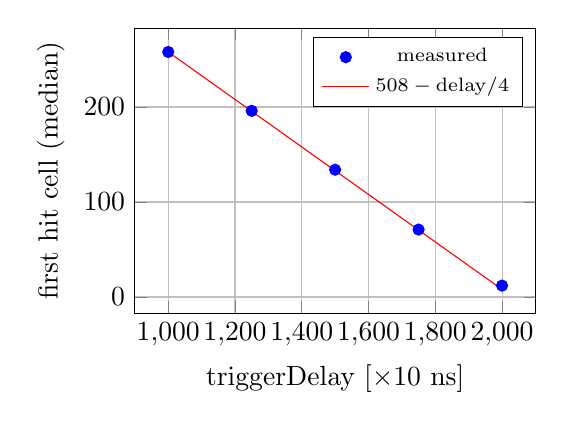
\begin{tikzpicture}
\begin{axis}[width=0.55\textwidth,height=5.2cm,xlabel={triggerDelay [$\times$10 ns]},ylabel={first hit cell (median)},grid=major,legend pos=north east,legend style={font=\scriptsize}]
\addplot[only marks,mark=*,blue] coordinates {(1000,258)(1250,196)(1500,134)(1750,71)(2000,12)};
\addlegendentry{measured}
\addplot[red,domain=1000:2000,samples=2] {508 - x/4};
\addlegendentry{$508 - \mathrm{delay}/4$}
\end{axis}
\end{tikzpicture}
\caption{S1: 帯の先頭セルと triggerDelay(run 78--82)。}
\end{figure}

\begin{table}[h]\centering\small
\caption{S1 triggerDelay(run 78--82)}
\begin{tabular}{rrrrrrrr}
\toprule
delay & run & first(p10--p90) & last(p90) & 先頭クリップ & ヒット ch & ok & 長さ [mm] \\
\midrule
1000 & 78 & 258 (243--264) & 282 (325) & 0 & 121 & 0.997 & 84.4 \\
1250 & 79 & 196 (182--201) & 220 (263) & 0 & 121 & 0.998 & 84.4 \\
1500 & 80 & 134 (119--139) & 157 (198) & 0 & 119 & 0.993 & 83.9 \\
1750 & 81 & 71 (55--76) & 94 (142) & 0.001 & 120 & 0.992 & 84.1 \\
2000 & 82 & 12 (3--16) & 31 (74) & \textbf{0.154} & 75 & \textbf{0.863} & \textbf{68.1} \\
\bottomrule
\end{tabular}
\end{table}

\subsection{peakingTime(S2)と応答核(S4)、デコンボリューション(S8)}
delay 1750、120 fC、GEM 250 × 3。長い整形ほど弱いストリップを拾う(ヒット ch 121 → 147)が飽和も増え、1014 ns では 1/3 のイベントが飽和する。
70 ns は S/N 不足で飛跡の 1/3 を失う。

\begin{table}[h]\centering\small
\caption{S2 peakingTime(run 83--86)}
\begin{tabular}{rrrrrrrrrr}
\toprule
peaking & run & 幅 [cell] & ヒット ch & 総電荷 & 飽和 & ok & 長さ / IQR & dEdx / IQR & 揺れ A0 [ADC] \\
\midrule
70 ns & 83 & 25 & 52 & 0.25 M & 0.0 \% & 0.660 & 45.4 / 46.3 & 4,602 / 855 & 4.4 \\
232 ns & 84 & 39 & 121 & 1.40 M & 0.3 \% & 0.998 & 85.2 / 58.4 & 12,493 / 6,438 & 12.4 \\
502 ns & 85 & 62 & 128 & 3.24 M & 4.8 \% & 0.997 & 88.9 / 58.8 & 19,087 / 9,466 & 27.9 \\
1014 ns & 86 & 106 & 147 & 7.21 M & 33.7 \% & 0.998 & 104.5 / 66.6 & 22,469 / 9,693 & 59.9 \\
\bottomrule
\end{tabular}
\end{table}

総電荷が 1 : 2.3 : 5.2 と peaking に比例して増えるのは、当初「短い整形は信号の一部しか積分していない」と読んだが、これは\textbf{誤り}で面積効果である(S8)。
\textbf{パルサー応答核}とは、電子回路(前置増幅器 + 整形器 + SCA)のインパルス応答のことである。AsAd には内蔵パルサーがあり、AGET の全 ch のテスト入力に同じ既知の電荷(階段電圧 $-300$ / $-100$ mV × 試験容量)を同時に注入できる。入力は検出器信号より十分に短い(事実上 δ 関数)ので、各 ch の出力波形をピーク時刻で揃えて平均し、ピークで規格化したものが核(kernel)になる(run 1 本で 68 ch × 4 AGET × 600 events ≈ 15 万波形の平均、図~\ref{fig:kernel})。検出器の波形は「電荷到着の時間分布 ⊗ 核」なので、核が分かれば逆畳み込みで電荷到着の時間分布に戻せる(S8)。測った核は 4 AGET で同一・無振動(1.8 µs 成分 ≤ 0.03 \%)で、ピーク利得比は 232 : 502 : 1014 = 1 : 1.05 : 1.17 である。
この核で α 波形を逆畳み込みすると(\texttt{deconv.C}、FFTW、λ$_\mathrm{rel}$ = 10$^{-3}$)、電荷比は 1 : 1.05 : 1.21 に戻り、パルサーの利得比と一致する。
すなわち\textbf{サンプル和の総電荷はどの peaking でも入力電荷を取り切っている}。逆畳み込み後の FWHM は 13.7 / 14.6 / 18.7 cell(0.55--0.75 µs)で検出器側の固有幅に収束する(図~\ref{fig:deconv})。
ノイズ増幅(S/N × 0.4--0.5)があるので運用には採らず、オフラインの選択肢(λ 10$^{-2}$)として残す。

また α 波形に見える周期 1.6--1.8 µs の「揺れ」(信号 ch のみ、電荷に比例)は、応答核に無いので AGET 整形系の応答ではない(起源は未解明、§\ref{sec:open})。

\begin{figure}[h]\centering
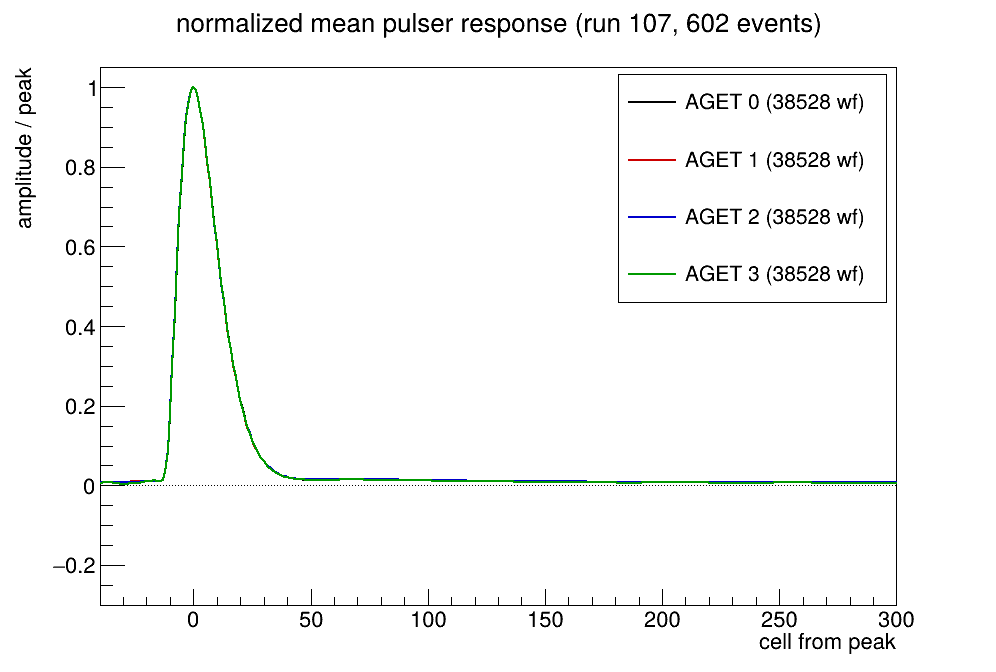
\includegraphics[width=0.48\textwidth]{fig/kernel2/run0107_kernel.png}\hfill
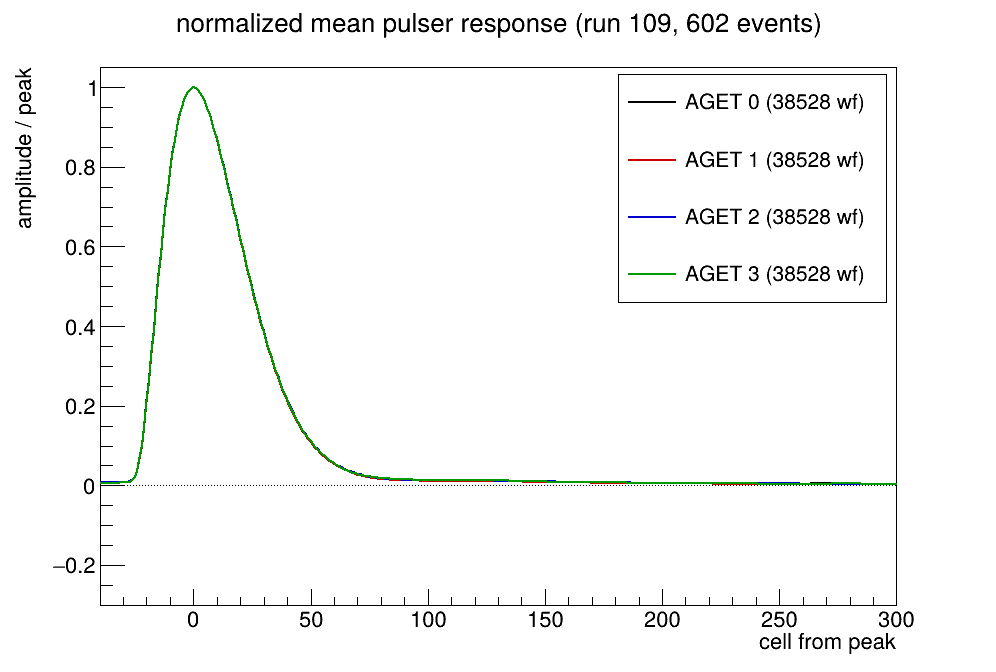
\includegraphics[width=0.48\textwidth]{fig/kernel2/run0109_kernel.png}
\caption{S4: パルサー応答核(左: 502 ns、run 107。右: 1014 ns、run 109)。4 AGET の平均波形をピークで規格化。無振動。}
\label{fig:kernel}
\end{figure}

\begin{figure}[h]\centering
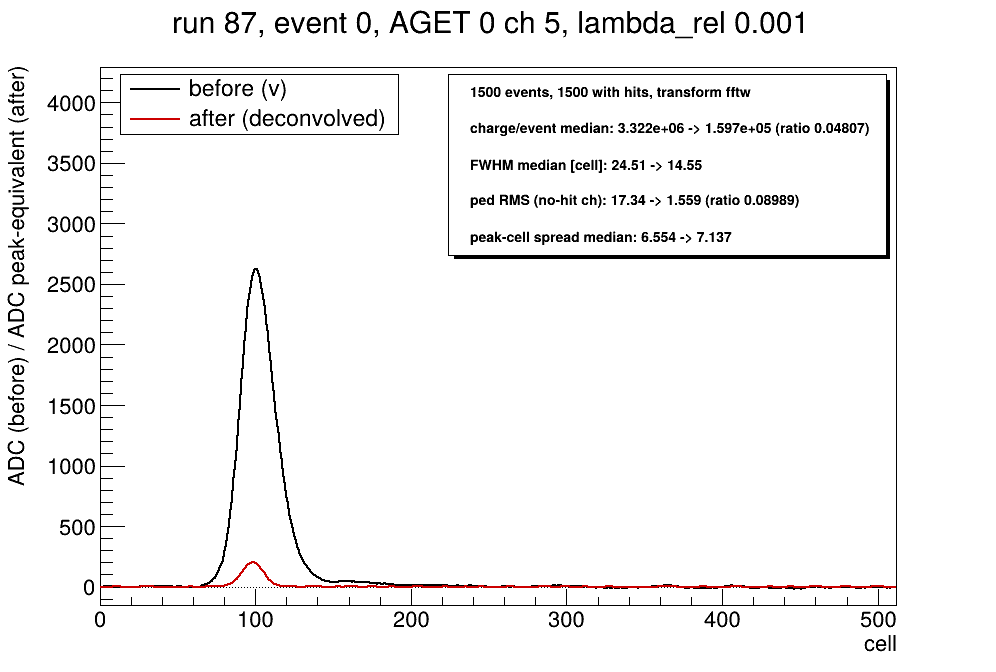
\includegraphics[width=0.6\textwidth]{fig/deconv/run0087_k107_l1e-3.png}
\caption{S8: run 87(502 ns × 120 fC)の 1 ch 波形の逆畳み込み前後。FWHM 24.5 → 14.6 cell、電荷比 0.048(核の和で規格化)。}
\label{fig:deconv}
\end{figure}

\subsection{gain(S3)と E 規則}
502 ns、GEM 250 × 3。E 規則「飽和 ch を含むイベント < 2 \% の中で最長の peaking とその gain」で \textbf{502 ns × 240 fC}(飽和 0.7 \%)を選んだ(GEM 250 × 3 のとき)。
1 pC は閾値 35 ADC で飛跡を失う(ok 0.009)。揺れの振幅は出力振幅に比例する(ゲインに乗る)。

\begin{table}[h]\centering\small
\caption{S3 gain(run 87--90, 112)}
\begin{tabular}{lrrrrrrrr}
\toprule
peaking × gain & run & ヒット ch & 総電荷 & 飽和 & クリップ 先/末 & ok & 長さ / IQR & dEdx / IQR \\
\midrule
502 × 120 fC & 87 & 127 & 3.20 M & 4.7 \% & 8.3 / 21.4 \% & 0.997 & 88.2 / 58.8 & 19,352 / 9,283 \\
\textbf{502 × 240 fC} & 88 & 119 & 1.71 M & \textbf{0.7 \%} & 2.7 / 8.9 \% & 0.991 & 84.0 / 59.3 & 11,946 / 5,896 \\
502 × 1 pC & 89 & 23 & 0.16 M & 0 \% & 0 / 0.1 \% & 0.009 & --- & --- \\
1014 × 1 pC & 90 & 43 & 0.53 M & 0 \% & 0 / 0.1 \% & 0.626 & 48.3 / 50.2 & 3,669 / 820 \\
1014 × 240 fC & 112 & 122 & 3.90 M & 2.1 \% & 0.7 / 4.8 \% & 0.998 & 84.6 / 58.4 & 16,155 / 7,814 \\
\bottomrule
\end{tabular}
\end{table}

\section{検出器の高電圧}

\subsection{GEM 電圧の余裕(S10)}
現地で GEM を 1 枚ずつ、または 3 枚同時に下げ(HV は GECO で手動、run は \texttt{gem\_point.sh})、同じ電子回路(502 ns × 120 fC)で総電荷を比べた。
図~\ref{fig:gain} のとおり、$\ln(Q/Q_0)$ は 3 枚の ΔV の合計で説明できる。箔ごとの傾きは GEM1 / GEM2 / GEM3 = 0.0148 / 0.0130 / 0.0145 ± 0.0026 /V で差は誤差内、
単独 3 点の和($-0.423 \pm 0.045$)と 3 枚同時($-0.425 \pm 0.026$)が一致するので加法性が成り立つ。平均の傾き $a = 0.0141 \pm 0.0015$ /V(GEM 合計 $-10$ V ごとに × 0.86)。
合計 $-30$ V(各 240 V、HIGS 本体と同じ値)まで、電子回路側で補って飛跡の質(ok、ヒット ch、長さ、dEdx の相対幅)は変わらず、トリップ・電流異常もなかった。
電流は全 ch 約 8.6--8.8 µA で、GEM の電圧を下げると電圧比どおりに下がる。HV 側の抵抗鎖(200 MΩ)は以前 Traian が回路図から説明したとおりで、今回の V--I の関係からも明確に言える: ch0--5 の合計電圧 1,770 V(240 × 3 時)/ 200 MΩ = 8.85 µA に対し実測 8.63--8.80 µA、250 × 3 時は 1,800 V → 9.0 µA に対し 8.80 µA。

\begin{figure}[h]\centering
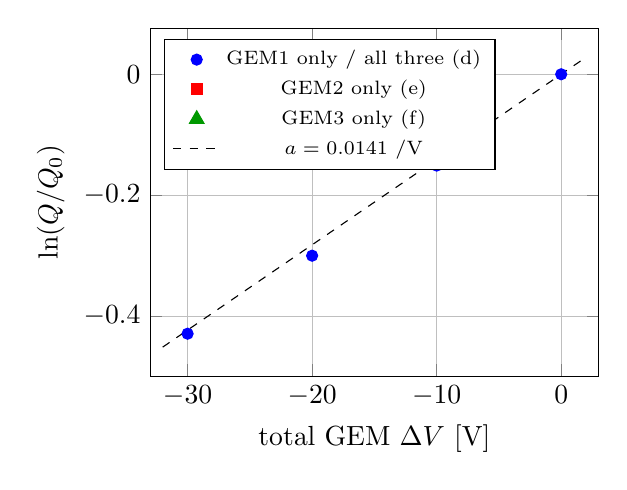
\begin{tikzpicture}
\begin{axis}[width=0.6\textwidth,height=6cm,xlabel={total GEM $\Delta V$ [V]},ylabel={$\ln(Q/Q_0)$},grid=major,legend pos=north west,legend style={font=\scriptsize},xmin=-33,xmax=3]
\addplot[only marks,mark=*,blue] coordinates {(0,0)(-10,-0.151)(-20,-0.300)(-30,-0.429)};
\addlegendentry{GEM1 only / all three (d)}
\addplot[only marks,mark=square*,red] coordinates {(-10,-0.130)};
\addlegendentry{GEM2 only (e)}
\addplot[only marks,mark=triangle*,green!60!black,mark size=3pt] coordinates {(-10,-0.145)};
\addlegendentry{GEM3 only (f)}
\addplot[black,dashed,domain=-32:2,samples=2] {0.0141*x};
\addlegendentry{$a = 0.0141$ /V}
\end{axis}
\end{tikzpicture}
\caption{S10: ゲインの法則。誤差は各点 ±0.026(1,500 events の電荷中央値)。}
\label{fig:gain}
\end{figure}

\begin{table}[h]\centering\small
\caption{S10 GEM 電圧(502 ns × 120 fC で比較。a は参照 run 87)}
\begin{tabular}{llrrrrrrr}
\toprule
点 & GEM1 / GEM2 / GEM3 [V] & run & ヒット ch & 総電荷 & 飽和 & ok & 長さ & dEdx / IQR \\
\midrule
a & 250 / 250 / 250 & 87 & 127 & 3.20 M & 4.7 \% & 0.997 & 88.2 & 19,352 / 9,283 \\
b & 240 / 250 / 250 & 122 & 124 & 2.76 M & 2.6 \% & 0.999 & 85.9 & 17,645 / 8,645 \\
c & 230 / 250 / 250 & 123 & 122 & 2.38 M & 1.1 \% & 0.997 & 84.7 & 15,258 / 7,697 \\
d & 240 / 240 / 240 & 126 & 121 & 2.09 M & 1.0 \% & 1.000 & 84.3 & 13,637 / 6,617 \\
e & 250 / 240 / 250 & 128 & 125 & 2.81 M & 2.0 \% & 0.996 & 86.3 & 17,553 / 8,318 \\
f & 250 / 250 / 240 & 129 & 123 & 2.76 M & 2.3 \% & 0.999 & 84.9 & 17,726 / 8,566 \\
\bottomrule
\end{tabular}
\end{table}

\subsection{ドリフト電圧(S12)}
運用点 B で DRIFT を 1,000 / 1,200 / 1,400 V(各 500 / 600 / 700 V × 2)にした。帯の時間幅 × V が一定(±6 \%)なので $v_\mathrm{drift} \propto E$ で、公称式 $v = 0.7233 \times E/p$ と矛盾しない。
パルス幅は 61 → 57 → 54 cell(E +40 \% で −11 \%、拡散の 1/√E に整形幅が足された形)。総電荷・ヒット ch は不変(GEM3 への集束に損失なし)。
$\sigma_z$ は cell では 1/v に比例するが \textbf{mm では一定(0.207 / 0.208 / 0.208)}。運用は 1,200 V のまま。

\begin{table}[h]\centering\small
\caption{S12 ドリフト電圧(run 130--132、運用点 B)}
\begin{tabular}{rrrrrrrrr}
\toprule
$V_\mathrm{drift}$ & run & 時間幅 [cell] & 時間幅 × V & パルス幅 [cell] & ヒット ch & 総電荷 & $\sigma_z$ [cell] & $\sigma_z$ [mm] \\
\midrule
1,000 & 131 & 28 & 28,000 & 61 & 120 & 2.07 M & 1.30 & 0.207 \\
1,200 & 130 & 22 & 26,400 & 57 & 121.5 & 2.09 M & 1.09 & 0.208 \\
1,400 & 132 & 20 & 28,000 & 54 & 123 & 2.09 M & 0.93 & 0.208 \\
\bottomrule
\end{tabular}
\end{table}

\subsection{運用点 B と一晩 run(S7、S16)}
2026-10-15 12:50 に \textbf{運用点 B}(GEM 240 × 3、502 ns × 120 fC、readout full、25 MHz、delay 1750、DRIFT 600 × 2、TR 350)を採用した。
GEM が 10 V/枚 低く、readout full で frameType 2(2 B/sample)なのでデータは A(partial、557 kB/event)の半分(278.8 kB/event)になる。
一晩 run(run 141、9.6 h、149,795 events、4.32 Hz、104 GB)の指標は 5.5 分の確認 run 130 と一致し、A の一晩(run 114、10 h、166,386 events)とも同等である。

\begin{table}[h]\centering\small
\caption{一晩 run の比較(S7、S16)}
\scriptsize\setlength{\tabcolsep}{3pt}
\begin{tabular}{llrrrrrrrrr}
\toprule
run & 設定 & events & kB/ev & ヒット ch & 総電荷 & 飽和 & ok & 長さ / IQR & $\sigma_z$ & $\sigma_{2D}$ \\
\midrule
114 & A 一晩(250×3、502 ns×240 fC、partial) & 166,386 & 557 & 119 & 1.71 M & 0.62 \% & 0.995 & 83.4 / 59.6 & 0.20 & 0.325 \\
130 & B 確認(5.5 分) & 1,500 & 278.8 & 121.5 & 2.09 M & 0.60 \% & 0.998 & 84.4 / 58.5 & 0.21 & 0.314 \\
\textbf{141} & \textbf{B 一晩} & 149,795 & 278.8 & 121 & 2.08 M & 0.92 \% & 0.999 & 84.1 / 58.8 & 0.20 & 0.321 \\
\bottomrule
\end{tabular}
\end{table}

\subsection{ガス流量(S19)}
運用点 B のまま、CO$_2$ の流量だけを 100 → 50 → 150 ml/min と変えた(チャンバー 54 L、91 mbar。run 174 = 100、175 = 50 で 67.7 h、176 = 150)。
\texttt{gas\_trend.C} で raw ツリーを 1 時間(175)/ 10 分(174、176)ビンに切り、イベント総電荷の中央値などの推移を見た(図~\ref{fig:gas})。

\begin{table}[h]\centering\small
\caption{S19 ガス流量(run 全体の指標。176 は 3 h 時点の暫定)}
\begin{tabular}{rlrrrrrrr}
\toprule
run & 流量 & events & ヒット ch & 電荷 & 飽和 & ok & 長さ / IQR & dEdx / IQR \\
\midrule
174 & 100 ml/min & 11,145 & 120 & 2.077 M & 1.0 \% & 0.999 & 84.1 / 58.9 & 13,532 / 6,508 \\
175 & 50 ml/min(67.7 h) & 1,057,719 & 120 & \textbf{2.002 M} & 0.9 \% & 0.999 & 83.8 / 58.9 & 12,998 / 6,336 \\
176 & 150 ml/min(暫定) & 50,335 & 121 & 2.085 M & 1.0 \% & --- & --- & --- \\
\bottomrule
\end{tabular}
\end{table}

\begin{figure}[h]\centering
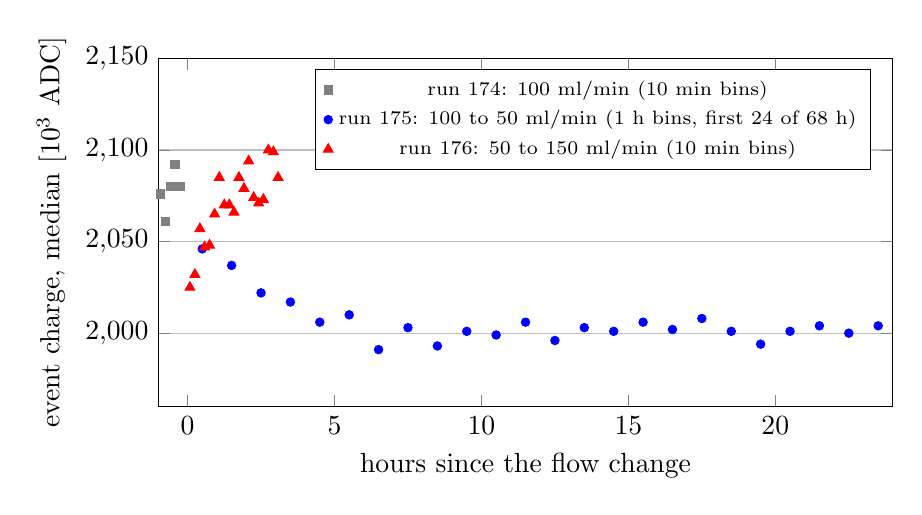
\begin{tikzpicture}
\begin{axis}[width=0.9\textwidth,height=6cm,xlabel={hours since the flow change},ylabel={event charge, median [$10^3$ ADC]},ymin=1960,ymax=2150,xmin=-1,xmax=24,ymajorgrids=true,legend pos=north east,legend style={font=\scriptsize}]
\addplot[only marks,mark=square*,gray,mark size=1.5pt] coordinates {(-0.92,2076) (-0.75,2061) (-0.58,2080) (-0.42,2092) (-0.25,2080)};
\addlegendentry{run 174: 100 ml/min (10 min bins)}
\addplot[only marks,mark=*,blue,mark size=1.5pt] coordinates {(0.50,2046) (1.50,2037) (2.50,2022) (3.50,2017) (4.50,2006) (5.50,2010) (6.50,1991) (7.50,2003) (8.50,1993) (9.50,2001) (10.50,1999) (11.50,2006) (12.50,1996) (13.50,2003) (14.50,2001) (15.50,2006) (16.50,2002) (17.50,2008) (18.50,2001) (19.50,1994) (20.50,2001) (21.50,2004) (22.50,2000) (23.50,2004)};
\addlegendentry{run 175: 100 to 50 ml/min (1 h bins, first 24 of 68 h)}
\addplot[only marks,mark=triangle*,red,mark size=2pt] coordinates {(0.08,2025) (0.25,2032) (0.42,2057) (0.58,2047) (0.75,2048) (0.92,2065) (1.08,2085) (1.25,2070) (1.42,2070) (1.58,2066) (1.75,2085) (1.92,2079) (2.08,2094) (2.25,2074) (2.42,2071) (2.58,2073) (2.75,2100) (2.92,2099) (3.08,2085)};
\addlegendentry{run 176: 50 to 150 ml/min (10 min bins)}
\end{axis}
\end{tikzpicture}
\caption{S19: 流量変更後の総電荷の推移。1 h ビンの統計精度は ±0.5 \%、10 min ビンは ±1 \%。run 175 は 24 h 以降 68 h まで 2.00 ± 0.01 M で平坦(昼夜の周期なし)。}
\label{fig:gas}
\end{figure}

\begin{itemize}
\item 50 ml/min にすると総電荷は 2.08 → 2.00 M(−3.5 \%)、dEdx も −4 \%。16 \% 点も同じ比で下がり、分布全体が一様に縮む。ヒット ch・飛跡長・ok・帯位置(first 75 / last 98 cell)・パルス幅(56 cell)は不変 = ドリフト速度と拡散は変わらない。HV(InfluxDB の 1 h 平均、69 点)は vmon ±0.05 V、imon ±0.5 \% で無関係。
\item 新しい平衡までの時間は数時間で、150 ml/min に戻したときの立ち上がりも約 0.5 h。これは 54 L を流量で入れ替える時定数(91 mbar で実流量は常温換算の 11 倍。50 ml/min: 1.6 h、150 ml/min: 0.54 h)に一致し、壁の脱離のような遅い過程は要らない。
\item 解釈: 不純物(主に H$_2$O、空気のリーク)の定常濃度は $c = c_\mathrm{bottle} + S/Q$($S$ = 系内の発生量、$Q$ = 流量)。ボンベ由来の項は流量に依らず差分に現れない。50 / 100 / 150 ml/min の 2.00 / 2.08 / 2.085 M は $S/Q$ に比例する形と 1 \% 以内で整合し、100 ml/min 以上では利得はほとんど変わらない。流量を変えたら \textbf{数時間は較正を跨がない}、流量を較正条件として記録する、の 2 点が運用の含意。
\item 付随: 長さ × 電荷の 2D で $^{228}$Th 系列の α 線が分離した(220Rn 6.29 MeV が 85 mm で停止、212Bi 45 mm、224Ra 25 mm、216Po / 212Po は 105 mm で突き抜け)。線源が 315 mm 外にあるため停止線の電荷 FWHM は 19--31 \% と悪い。圧力スキャン(次期)の指標の土台。
\end{itemize}

\section{ヒットの精度}

\subsection{z 残差(S11)}
直線に対するヒットの z 残差(図~\ref{fig:resid})の robust σ は 232--502 ns で \textbf{0.19--0.22 mm ≈ 1 cell}(1 cell = 40 ns × 4.77 mm/µs = 0.19 mm)。
1014 ns で 0.25--0.31 mm(+30--60 \%)、70 ns で 0.27 mm(S/N 不足)。HV(GEM 250 → 230、配分)には依らない(0.20--0.22)。
S12 とあわせると \textbf{$\sigma_z$ は時間でなく距離の精度で決まっている}(候補: ストリップ幅 × 飛跡の傾き ≈ 0.18 mm)。
1014 ns の悪化分は電子回路の時間精度が二乗で足されたもの($\sqrt{0.31^2 - 0.21^2} \approx 0.23$ mm)。
RMS は robust σ の 2--5 倍で裾が重いので、当てはめは robust に行う必要がある。
なお「パルス幅を z の誤差に使えないか」は Aogaki の思いつきを検証したもので(他で行われている手法ではない)、結果は\textbf{10 倍以上過大}(固有幅 14.5 cell = 2.8 mm、生の幅 7--20 mm に対し実測 0.2 mm)だった。

\begin{figure}[h]\centering
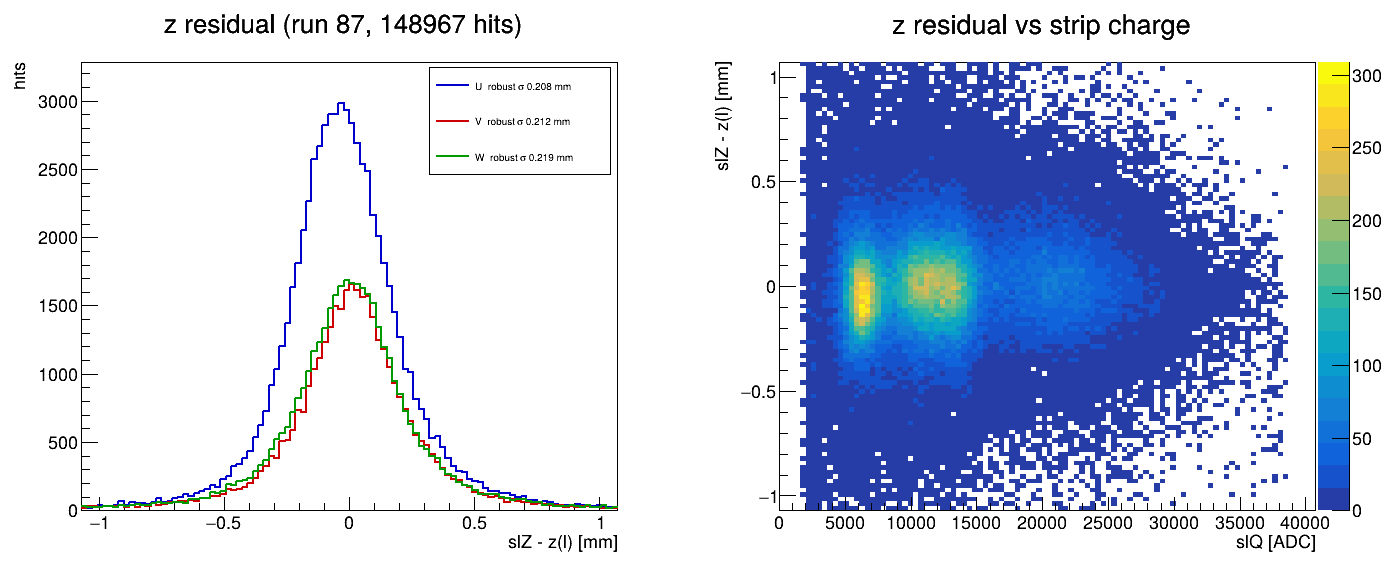
\includegraphics[width=0.95\textwidth]{fig/resid/run0087_resid.png}
\caption{S11: run 87(502 ns)のヒット z 残差(左: U/V/W、robust σ 0.21--0.22 mm。右: ストリップ電荷との相関)。}
\label{fig:resid}
\end{figure}

\subsection{2D 重心精度 = U/V/W 閉合残差(S14)}\label{sec:closure}
同じ z スライス(1 cell)で、U・V・W の各ストリップ面(view)ごとに電荷重心のストリップ位置 $s_U$, $s_V$, $s_W$ を取ると、3 方向が 60° ずつなので和 $s_U + s_V + s_W$ は幾何的に定数になるべきである。そのばらつき(閉合残差)の robust σ を $\sqrt{3}$ で割ったものが「1 view あたり」= 1 方向のストリップ群で測った重心の精度である(ヒット ch 条件 + 時間窓 |t − t$_\mathrm{peak}$| ≤ 15 cell)。
\textbf{232 ≈ 502 ns で 0.30 mm/view が最良}、1014 ns は 0.39--0.43(パルスが広く窓からはみ出す)、70 ns は 1.1 mm。HV には依らず(0.30--0.32)、DRIFT 1,000 V でわずかに悪い(0.34)。
電荷依存が強く(Q1 0.7--0.8 → Q4 0.40--0.45 mm)、2D 精度は S/N で決まる。

まとめ: 運用点 B(502 ns)でのヒット(z スラブ)の誤差は \textbf{$\sigma_s \approx 0.30$ mm(2D、view ごと)、$\sigma_z \approx 0.20$ mm}。

\begin{figure}[h]\centering
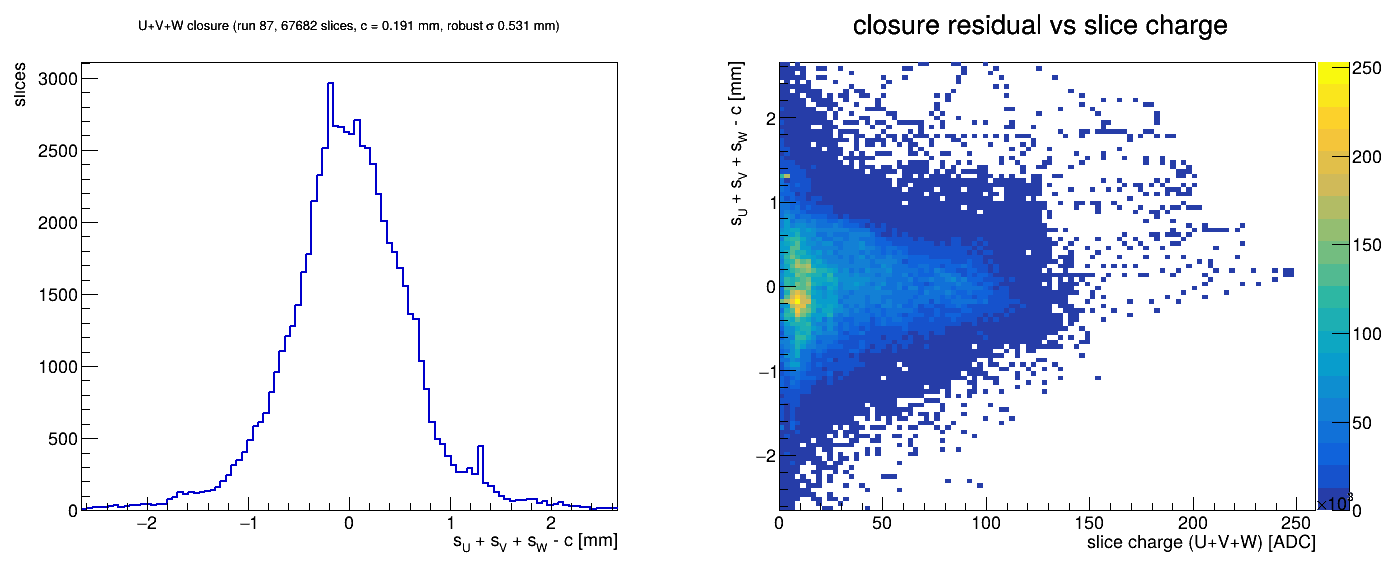
\includegraphics[width=0.95\textwidth]{fig/closure/run0087_closure.png}
\caption{S14: run 87 の閉合残差(左: 分布、robust σ 0.53 mm → /√3 = 0.31 mm/view。右: スライス電荷との相関)。}
\label{fig:closure}
\end{figure}

\section{読み出し方式・レート・ゼロサプレッション}

\subsection{readout と hit register(S9、S15)}
現用だった partial readout は、テンプレートの \texttt{channel Reading = always} のため全 ch を読んでおり、hit register の閾値は無効だった。
しかも partial は frameType 1(4 B/sample)で、full(frameType 2、2 B/sample、279 kB/event)の \textbf{2 倍}(557 kB/event)のデータになる。
\texttt{Reading = only\_if\_hit} のテンプレート(S15)では閾値が効く(global / lsb を上げると 400 → 241 kB)が、4 B/sample のため full 比で最大 14 \% しか減らない。
よって\textbf{通常運用は full}とし、圧縮は ZS に任せる。

\subsection{最大レート(S17)}
周期トリガ(信号なし)と AsAd パルサー(全 256 ch に $-300$ mV = 占有率 100 \%)で上限を測った。
\begin{itemize}
\item \textbf{上限は zCoBo FW の読み出し時間}: 272 ch で 2.94 ms(≈ 340 Hz、1 AsAd)。full でも ZS でも同じ。事象間隔は「周期 + 2.94 ms」で一定で、網の背圧による乱れはない。
\item \textbf{読み出し中のトリガは失われる}(キューされない): パルサー 2 ms 周期 → 1 個おき。不感時間 = レート × 読み出し時間(ビーム 100 Hz では full で 29 \%)。
\item \textbf{読み出し時間 ≈ 0.11 ms + 10.4 µs × 読む ch 数}: hit partial で信号なし(FPN 16 ch)なら 0.28 ms(779 Hz)。α 事象(≈ 136 ch)なら ≈ 1.5 ms → 100 Hz で 15 \%。\textbf{不感時間を縮める手段は hit register partial だけ}。
\item \textbf{ZS はバイトだけを減らす}(読み出し時間は不変)。全 ch ヒットでも 65 kB。partial + ZS は両立する(frameType 1 + ZS)。
\item 1 GbE は full なら 340 Hz まで余裕(1 ms パルサーで 86 MB/s、縁)。partial で全 ch ヒットだと 557 kB で 170 Hz 止まり。光 / 10 GbE は zCoBo のリンク(FW の MAC が 1 GbE)には効かない。
\end{itemize}

\begin{table}[h]\centering\small
\caption{S17 最大レート(run 148--169)}
\footnotesize
\begin{tabular}{llrrrl}
\toprule
系列 & 信号 & 達成 [Hz] & 事象間隔の下限 [ms] & kB/event & 限界 \\
\midrule
B full(272 ch) & なし / パルサー全 ch & 254 / 310 & 周期 + 2.94 & 279 & FW 読み出し \\
hit partial g4 & なし(FPN 16 ch) & 779 & 周期 + 0.28 & 33 & FW 読み出し(ch 数に比例) \\
hit partial g4 & パルサー全 ch(frameType 1) & 170 & 3.0 + stall & 557 & \textbf{1 GbE} \\
ZS ch ごと & パルサー全 ch & 333 & 3.0 & 65 & FW 読み出し \\
hit partial + ZS & パルサー全 ch & 333 & 3.0 & 65 & FW 読み出し \\
\bottomrule
\end{tabular}
\end{table}

\subsection{ゼロサプレッション(S5、S13、S18)}
pedestal run(periodic トリガ、full、150 events)から ch ごとの平均と σ の表を作り(S5: 信号 ch の ped 中央値 456.5 ADC、σ 中央値 7.6--8.0、FPN σ 3.3)、
閾値 = ped + 5σ を ch ごとの exceptions として params に入れた(\texttt{zs\_params.sh})。
ZS データは閾値未満のサンプルが存在しないので、波形からペデスタルを取る従来の算法(TPCReco の \texttt{PedestalCalculatorGRAW} も、ユーザーの macros も)は壊れる。
DAQ 側では同じ表を \texttt{[system] ped\_table} に置き、root\_sink(PEventTPC の表モード)・monitor(Event Display の復元)・解析マクロ(\texttt{zs\_restore.C} で抑制セルを表の値で埋めた同名 raw を作り macros を無改造で通す)の 3 経路で対応した(SPEC v1.49)。

検証 run(S18、各 1,500 events、運用点 B の電子回路)の結果を表~\ref{tab:zs} に示す。
\textbf{ZS は品質を落とさない}(ヒット ch、ok、長さ、dEdx IQR、$\sigma_z$、$\sigma_{2D}$ が基準と同じ。総電荷は閾値未満の裾の分 −3 \%)。
FPN を残しても指標は 1 つも改善せず +32 kB/event なので \textbf{FPN は抑制}する。
ZS が本質的に影響し得る唯一の処理は、閾値未満の裾を使う波形処理(§2.2 のデコンボリューションや Unfolding)で、ヒット・飛跡・電荷の指標には効かない。hit partial g4 + ZS は最小(23.1 kB、1/12)で、ヒット ch −4、$\sigma_{2D}$ +12 \% の小さな代償がある。不感時間を縮められるのはこれだけなので、
\textbf{ビーム run の既定候補 = hit g4 + ZS(FPN 抑制)}、線源 run は B full(現行)か B + ZS とした。

\begin{table}[h]\centering\small
\caption{S18 ZS 検証(run 170--173、基準 = run 130)}
\label{tab:zs}
\footnotesize
\begin{tabular}{rlrrrrrrr}
\toprule
run & 設定 & kB/event & ヒット ch & 総電荷 & ok & 長さ & $\sigma_z$ & $\sigma_{2D}$ \\
\midrule
130 & B full(基準) & 278.8 & 121.5 & 2.09 M & 0.998 & 84.4 & 0.21 & 0.314 \\
\textbf{170} & \textbf{B + ZS} & \textbf{30.9} (1/9) & 121 & 2.02 M & 0.998 & 83.9 & 0.20 & 0.320 \\
171 & B + ZS、FPN 残し & 63.1 & 120 & 2.03 M & 0.997 & 83.2 & 0.20 & 0.319 \\
\textbf{172} & \textbf{hit g4 + ZS} & \textbf{23.1} (1/12) & 117 & 2.03 M & 0.996 & 82.9 & 0.19 & 0.357 \\
173 & hit g4 + ZS、FPN 残し & 55.7 & 116 & 1.99 M & 0.997 & 82.0 & 0.19 & 0.354 \\
\bottomrule
\end{tabular}
\end{table}

\begin{figure}[h]\centering
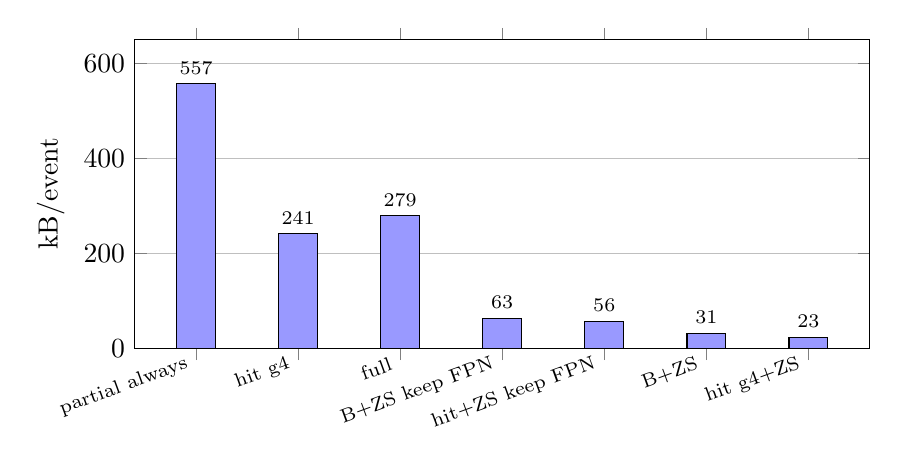
\begin{tikzpicture}
\begin{axis}[ybar,width=0.9\textwidth,height=5.5cm,ylabel={kB/event},symbolic x coords={partial always,hit g4,full,B+ZS keep FPN,hit+ZS keep FPN,B+ZS,hit g4+ZS},xtick=data,x tick label style={font=\scriptsize,rotate=20,anchor=east},nodes near coords,nodes near coords style={font=\scriptsize},ymin=0,ymax=650,bar width=14pt,ymajorgrids=true]
\addplot[fill=blue!40] coordinates {(partial always,557)(hit g4,241)(full,279)(B+ZS keep FPN,63)(hit+ZS keep FPN,56)(B+ZS,31)(hit g4+ZS,23)};
\end{axis}
\end{tikzpicture}
\caption{α 事象 1 イベントあたりのデータ量(S9、S15、S18)。}
\end{figure}

\subsection{ビーム run(≈ 100 Hz)に向けた設計}
ビーム run は周期トリガではなく、\textbf{粒子の到来がランダム}で期待レート ≈ 100 Hz(もっと出れば歓迎)という想定である。ランダム到来では読み出し時間 τ が非麻痺型の不感時間として効き、受理レートは $m = n/(1 + n\tau)$ になる(表~\ref{tab:deadtime})。
100 Hz でも full なら 1/4 を落とすので、hit partial の価値は周期ビームより大きい。受理レートは $1/\tau$ で飽和する(full 340 Hz、partial ≈ 680 Hz)。帯域は ZS で 23 kB × 300 Hz ≈ 7 MB/s なので問題にならない。

\begin{table}[h]\centering\small
\caption{ランダム到来での受理レート $m = n/(1+n\tau)$}
\label{tab:deadtime}
\begin{tabular}{rrr}
\toprule
真のレート $n$ & full(τ = 2.94 ms) & hit partial(τ ≈ 1.5 ms、α 相当 136 ch) \\
\midrule
100 Hz & 77 Hz(−23 \%) & 87 Hz(−13 \%) \\
200 Hz & 127 Hz(−37 \%) & 154 Hz(−23 \%) \\
300 Hz & 160 Hz(−47 \%) & 207 Hz(−31 \%) \\
飽和 & 340 Hz & ≈ 680 Hz \\
\bottomrule
\end{tabular}
\end{table}

\textbf{不感時間の実測が要る。} zCoBo は読み出し中に来たトリガに eventIdx を付けない(受理したトリガだけが連番になる)ので、落とした数はデータから分からず、収量の不感時間補正ができない。外部トリガの生パルスをスケーラで run ごとに数える(zCoBo の SMA OUT1 = ラッチ時のパルスも同じスケーラで数えれば受理数と比較できる)、DAQ 側は「0.11 ms + 10.4 µs × 読み出し ch 数」から τ を推定して run ごとに記録する(TODO/131 B-5)。

\textbf{10 GbE について。} zCoBo(ZC706)の 2 つのポートはどちらも 10 GbE にならない。RJ45 側は Zynq PS の固定 MAC(1 Gb/s まで、FW では 100 Mbit の管理用)。SFP+ 側は GTX トランシーバで HW 的には 10 Gb/s 可能だが、FW が PL に 1G の AXI Ethernet コア(1000BASE-X、ライン速度 1.25 Gb/s)を置き、ARM 上の Linux の TCP で送っている(FW パッケージの boot log・README で確認)。したがって光モジュール(1000BASE-SX/LX)は銅アダプタと同じく問題なく使えるが速度は 1 GbE のままで、10G 専用のモジュールを挿しても 10G にはならない(1G 非対応品はリンクしない)。
10G 化には FW の作り直し(有償 10G IP + PL 側 TCP/UDP エンジン)が要り、しかも上限は読み出し時間 2.94 ms の方が先に効く。この 2.94 ms は AGET 仕様(読み出しクロック 25 MHz で 512 cell × 68 ch ≈ 1.4 ms/AGET)の約 2 倍で、読み出し系の FW に余地がある可能性がある — Warsaw に「AGET の読み出しクロック」を聞く価値がある。

ELITPC(Warsaw、zCoBo 2 枚 × 2 AsAd)の見積もり: 1 枚 544 ch → 読み出し ≈ 5.8 ms → full では飽和 170 Hz・100 Hz ランダムで −37 \%。partial(占有 25 \%、≈ 150 ch)なら ≈ 1.7 ms → −15 \%。
帯域は full で 1 GbE の縁(95 MB/s)、partial + ZS なら余裕。\textbf{ビーム 100 Hz の設計 = hit register partial + ZS + 2 本の 1 GbE(PC 側 10 GbE に集約)+ トリガのスケーラ}。FW の読み出し時間が 2 AsAd で本当に 2 倍かは Warsaw で要実測。
注意: ZS graw はオフラインの grawToEventTPC のペデスタル計算を壊すので、Warsaw で ZS を使うなら「我々の PEventTPC(表で減算済み)を使う」か「TPCReco に表の入力を足す」かを先方と決める必要がある。

\section{未解決と次の課題}\label{sec:open}
\begin{itemize}
\item \textbf{ドリフト端(S6)}: 12.5 MHz・窓 41 µs でも α 飛跡はトリガから 2--4 µs に収まる(図~\ref{fig:drift})。現在の線源はチャンバーの外(ガス配管に連結した位置)にあり、立体角の都合で飛跡の z 方向の広がりはほぼ変わらないので、今の配置では陰極(20 cm)側まで届く飛跡は得られない。$v_\mathrm{drift} = L / t_\mathrm{max}$ の絶対値は、線源を再びチャンバー内に入れたときに測る。cell 340 付近の山は窓位置に依らず物理ではない(未解明)。
\item \textbf{ガスの不純物源}: 流量依存(S19)の $S$ がリークか壁の脱離かは未分離。温度・圧力の記録(環境センサ)と、線源を中に入れてからの電荷 vs ドリフト時間で切り分ける。
\item \textbf{揺れ}: α 波形の周期 1.6--1.8 µs の成分(信号 ch のみ、電荷に比例)。AGET の応答核には無い。検出器側(GEM / 誘導)の可能性。
\item \textbf{複数飛跡}: 現在の再構成は 1 イベント = 直線 1 本。502 ns で RMS が 1014 ns より大きい(外れ値の出方の違い)の素材でもある。
\item \textbf{ZS の run ごとのカウンタ}(TODO/159): root\_sink / monitor の ZS カウンタを run\_stop に出す。PEventTPC 側の電荷和の照合も未実施。
\end{itemize}

\begin{figure}[h]\centering
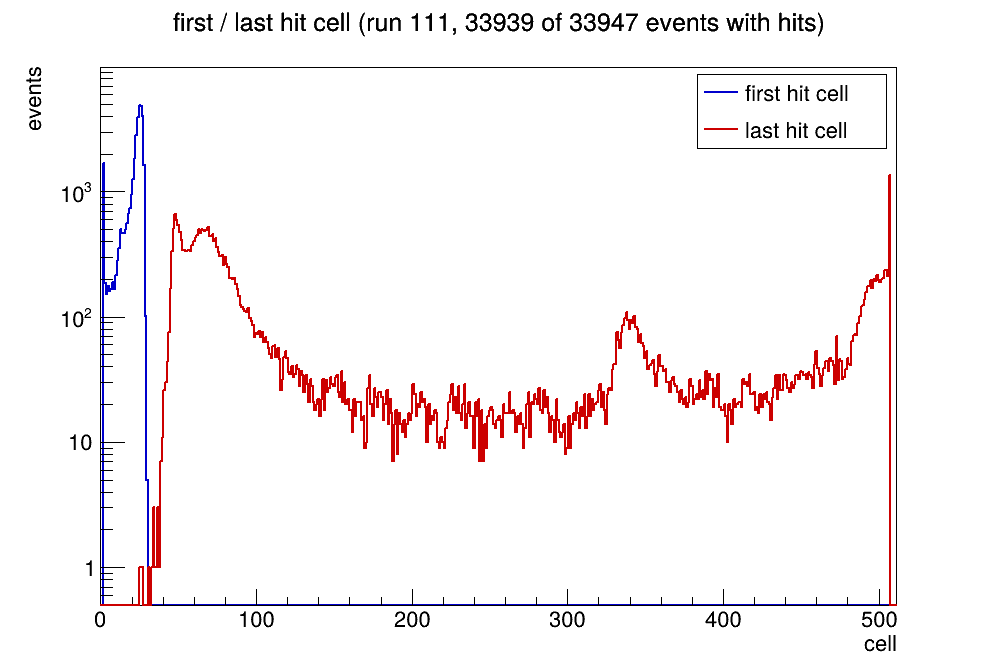
\includegraphics[width=0.6\textwidth]{fig/drift/run0111_drift.png}
\caption{S6: run 111(12.5 MHz、delay 3800)の first / last hit cell。last hit は 50--100 cell(トリガから 2--4 µs)に集中し、cell 508 のスパイクは窓端の跳ね。}
\label{fig:drift}
\end{figure}

\FloatBarrier
\appendix
\section{道具と記録の所在}
\begin{itemize}
\item リポジトリ: \url{https://github.com/aogaki/tpcdaq-rs}。DAQ のソース(Rust + C++)、仕様書、運用手順、スキャン台帳、チケット(設計の経緯と結果)がすべてここにある。開発者向けの文書は日本語だけなので、興味があって英語版が要る場合は Aogaki に言ってもらえれば LLM 翻訳を用意する。
\item 台帳: \texttt{docs/SCANS\_ja.md}(S1--S18、数字の正)。経緯と判断: \texttt{TODO/archive/135--158}。
\item 道具: \path{tools/scan/}(\sloppy \texttt{scan.py}、\texttt{run\_metrics.C}、\texttt{metrics\_for\_run.sh}、\texttt{pulser\_kernel.C}、\texttt{deconv.C}、\texttt{drift\_end.C}、\texttt{hit\_residuals.C}、\texttt{uvw\_closure.C}、\texttt{zs\_exceptions.py}、\texttt{zs\_params.sh}、\texttt{zs\_restore.C}、\texttt{ledger.py})。各マクロにテストあり。
\item 仕様: \texttt{docs/SPEC\_ja.md} v1.49(ZS 表モード、0x02 復元、ped\_table、decoder カウンタ、§13-9)。運用: \texttt{docs/RUNBOOK\_ja.md}「ZS 運用」。
\item ELITPC: データ \path{/data/tpcdaq/run00NN/}、指標 \path{~/test/scan/metrics/}、図 \path{~/test/scan/}\{resid, closure, kernel2, deconv, drift\}、較正表 \path{~/test/scan/calib/pedestal_232ns.json} / \path{pedestal_502ns.json}。
\end{itemize}

\section{運用点 B の params}
\texttt{base\_1750.json}(ELITPC \texttt{\textasciitilde/test/scan/})。knobs: \texttt{writingClockFrequency\_MHz} 25、\texttt{triggerDelay} 1750、\texttt{triggerMode} external、\texttt{peakingTime\_ns} 502、\texttt{gain} 120 fC、\texttt{readout} full、\texttt{fpnRead} true、\texttt{zeroSuppression.enabled} false。
ビーム候補: テンプレート \texttt{configure-elinp-hit.xcfg}(\texttt{channel Reading only\_if\_hit})、global 4 / lsb 15、ZS 有効 + \texttt{pedestal\_502ns.json} の exceptions(FPN 閾値 4095)。
\end{document}
